%\documentclass{article}
\documentclass{report} % Use the custom report.cls style

\usepackage[left=0.75in,top=0.6in,right=0.75in,bottom=1.0in]{geometry} % Document margins
\usepackage[utf8]{inputenc}

\usepackage{graphicx} 
\usepackage{float}
\usepackage{subfigure}

\title{\textbf{The reading paper on agent in artificial intelligence}}
\author{Kan, Hao-Cheng}
\date{6 October,2021}

\begin{document}

\maketitle

%\section{Introduction}

\section{Summary}

This research responds to the recent proposal of multi-agent reinforcement learning, and is full of great potential in terms of further application on the Internet. The authors of this research want to combine this with the game theory.

The researcher attempts to use game theory to first analyze the solutions generated by using different information structures created by the network multi-agent systems; the types of information shared between these information structures; the relationship between the used communication protocol and the network topology.

The interesting part of this study is that every part of the game theory is related to the network system, which is equivalent to perfect integration of the game theory, which is a part of microeconomics, and the reinforcement learning in deep learning, and the study is then integrated into the network system.

\section{Strengths}

I personally feel that game theory has many opportunities to be applied in deep learning. This research provides an interesting idea for deep learning.
 
\section{Weaknesses}

The research currently only uses water resource systems to represent the system of a network traffic, and it may be necessary to build a large-scale network system to verify the actual operations.

\section{Detailed comments}

I think that in the past, this issue was widely used in microeconomics to discuss issues regarding public finances. For example, the herders living on the grassland tried to pursue the maximization of their own interests, which eventually led to the depletion of the grassland. Another example is the marine fishery resources. The individual fishermen also pursued the maximization of their own interests in fishery, which was also responsible for the disappearance of fishing resources. This theory can even be used to analyze issues regarding upstream and downstream manufacturers and some externalities, such as the discharge of wastewater from upstream steel plants and fishery problems caused in downstream.

This concept is also applied in system design, such as ability allocation on online game systems. Players of equal strength can join the same battle, so that players can get a better gaming experience. As a result, the player is more willing to spend more time in the game. In this research, game theory is used to discuss issues regarding resource control in network systems, such as network bandwidth, the allocation of computing resources, and the allocation of memory.

If possible, I would like to try different methods and add other different methods for analysis on each node of the system to improve the overall efficiency.

\section{Figures}

It can be seen that the system uses the water resource system to represent the operation of the network system in the flow share control.
\begin{figure}[H]
\centering 
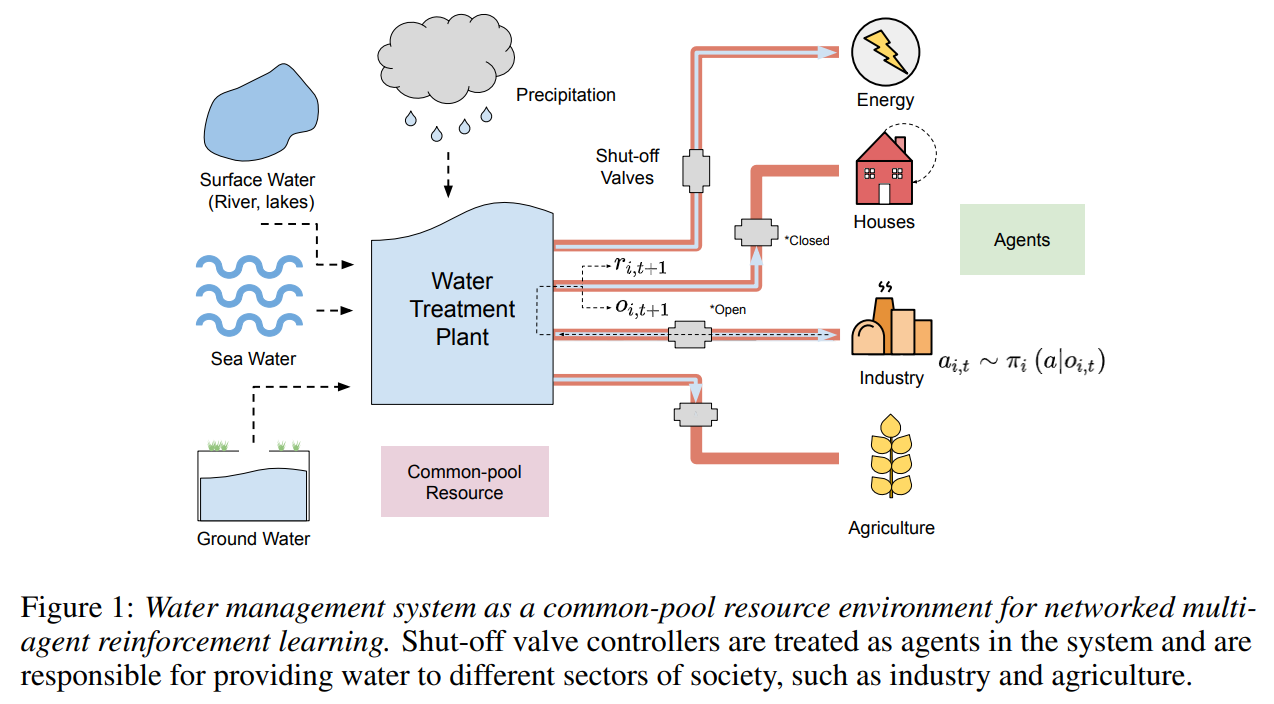
\includegraphics[width=0.7\textwidth]{re-ai-1.png} 
\caption{Figure 1}
\label{Report.1}
\end{figure}
\begin{figure}[H]
\centering 
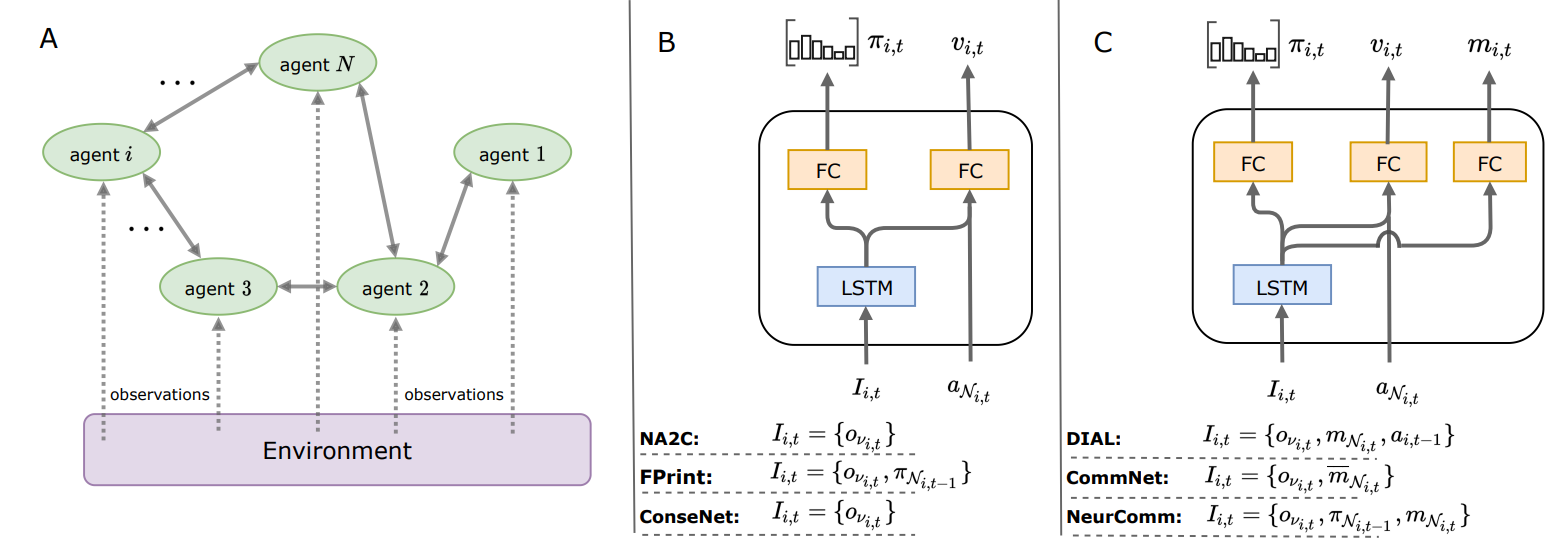
\includegraphics[width=0.7\textwidth]{re-ai-2.png} 
\caption{Figure 2}
\label{Report.2}
\end{figure}
\end{document}
